\documentclass[pdflatex,compress]{beamer}

%\usetheme[dark,framenumber,totalframenumber]{ElektroITK}
\usetheme[darktitle,framenumber,totalframenumber]{ElektroITK}

\usepackage{graphicx}
\usepackage{multicol}
\usepackage[bahasai]{babel}

\title{METODE NUMERIK}
\subtitle{Solusi Persamaan Nirlanjar}

\author{Tim Dosen Pengampu}

\begin{document}
	
\maketitle

\section{Pengantar}

\begin{frame}
	\frametitle{Pengantar}
	\begin{itemize}
		\item Engineer berhadapan dengan persoalan mencari solusi persamaan/ akar persamaan.
		\item Contoh mudah: $ 2x - 3 = 0 $, sehingga $ x = 3/2 $.
		\item Permasalahan yang muncul dalam bentuk nirlanjar (non linear).
		\item Contoh:
		\begin{itemize}
			\item Suatu arus osilasi dalam rangkaian listrik diberikan oleh \[ I = 10 e^{-t} \sin(2\pi t) \]
			\item Tentukan semua nilai $ t $ sedemikian sehingga $ I = 2 $ Ampere 
		\end{itemize}
		\item Contoh di atas memperlihatkan bentuk persamaan yang rumit yang tidak bisa dipecahkan secara analitik.
		\item Sehingga menggunakan metode numerik.
	\end{itemize}
\end{frame}
\begin{frame}
	\frametitle{Rumusan Masalah}
	\begin{itemize}
		\item \textbf{Persoalan:} Temukan nilai $ x $ yang memenuhi persamaan
		\[f(x) = 0\]
		yaitu nilai $ x = s $ sedemikian sehingga $ f(s) = 0 $.
		\item Nilai $ x = s $ disebut \textbf{akar} persamaan $ f(x) = 0 $
	\end{itemize}
\end{frame}

\section{Metode Pencarian Akar}

\begin{frame}
	\frametitle{Metode Pencarian Akar}
	\begin{enumerate}
		\item Metode tertutup (bracketing method)
		\begin{itemize}
			\item Mencari akar di dalam selang $ [a, b] $.
			\item Selang $ [a, b] $ sudah dipastikan berisi minimal satu buah akar.
			\item Karena itu metode jenis ini selalu berhasil menemukan akar.
			\item Dengan kata lain, iterasinya selalu konvergen (menuju) ke akar,
			\item Karena itu metode tertutup kadang-kadang dinamakan juga \textbf{metode konvergen}.
		\end{itemize}
	\end{enumerate}
\end{frame}

\begin{frame}
	\begin{enumerate}
		\setcounter{enumi}{1}
		\item Metode terbuka
		\begin{itemize}
			\item Tidak memerlukan selang $ [a, b] $ yang mengandung akar.
			\item Mencari akar melalui suatu iterasi yang dimulai
			dari sebuah tebakan (\textit{guest}) awal.
			\item Pada setiap iterasi kita menghitung hampiran akar yang baru.
			\item Mungkin saja hampiran akar yang baru mendekati akar sejati (konvergen), atau mungkin juga menjauhinya (divergen).
			\item Karena itu, metode terbuka tidak selalu berhasil menemukan akar, kadang-kadang konvergen, kadangkala ia divergen.
		\end{itemize}
	\end{enumerate}
\end{frame}

\section{Metode Tertutup}

\begin{frame}
	\frametitle{Metode Tertutup}
	\begin{itemize}
		\item Diperlukan selang $ [a, b] $ yang mengandung minimal satu buah akar.
		\item Syarat cukup keberadaan akar: Jika $ f(a) f(b) < 0 $ dan $ f(x) $ menerus di dalam selang $ [a, b] $, maka paling sedikit terdapat satu buah akar persamaan f(x) = 0 di dalam selang $ [a, b] $.
		\item Dengan kata lain: selang $ [a, b] $ harus berbeda tanda pada nilai-nilai fungsinya supaya terdapat minimal 1 buah akar.
	\end{itemize}
\end{frame}

\begin{frame}
	\frametitle{Syarat cukup keberadaan akar}
	\begin{center}
		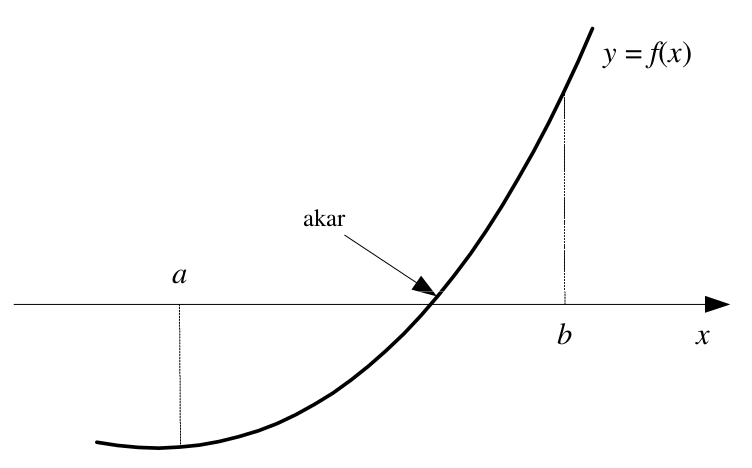
\includegraphics[width=1\linewidth]{img/img01}
	\end{center}
\end{frame}

\begin{frame}
	\frametitle{Kondisi yang mungkin terjadi}
	\begin{enumerate}
		\item $ f(a)f(b) < 0 $, maka terdapat akar sebanyak bilangan ganjil.
		\begin{center}
			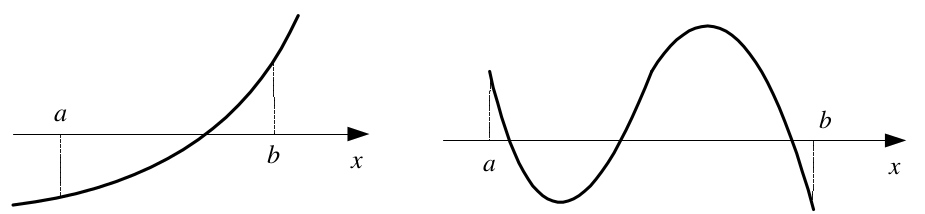
\includegraphics[width=0.8\linewidth]{img/img02}
		\end{center}
		\item $ f(a)f(b) > 0 $, maka terdapat akar sebanyak bilangan genap (termasuk tidak ada akar).
		\begin{center}
			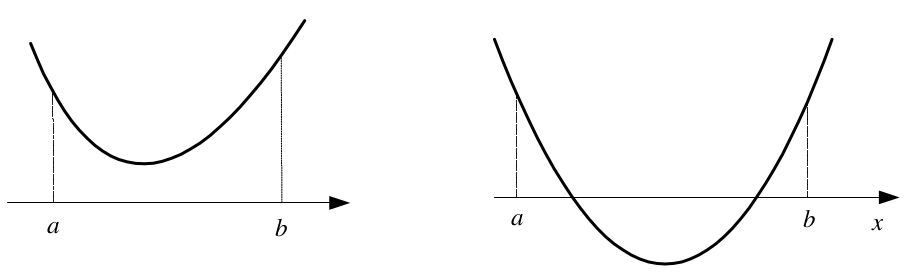
\includegraphics[width=0.8\linewidth]{img/img03}
		\end{center}
	\end{enumerate}
\end{frame}

\begin{frame}
	\begin{itemize}
		\item Cara menentukan selang yang cukup kecil dan mengandung akar:
		\begin{enumerate}
			\item Membuat grafik fungsi di bidang X-Y, lalu melihat di mana perpotongannya dengan sumbu-X.
			\item Membuat tabel yang memuat nilai-nilai fungsi pada pada titik-titik absis yang berjarak tetap (h).Nilai h dibuat cukup kecil. (lihat contoh berikut)
		\end{enumerate}
	\end{itemize}
\end{frame}

\begin{frame}
	\begin{itemize}
		\item \textbf{Contoh:} Tabel nilai-nilai $ f(x) = e^x - 5x^2 $ mulai dari $ a = -0.5 $ sampai $ b = 1.4 $ dengan kenaikan absis sebesar $ h = 0.1 $		
	\end{itemize}
	\begin{multicols}{2}
	\begin{center}
		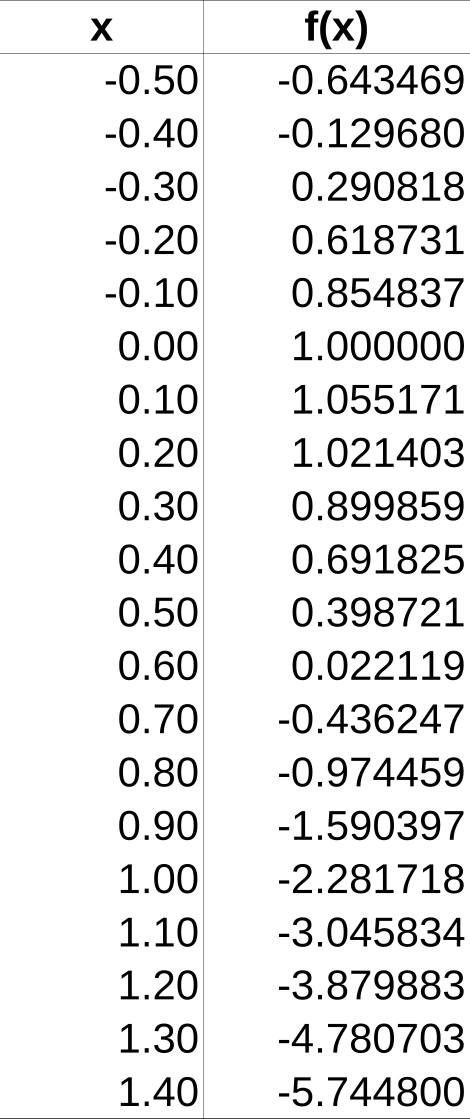
\includegraphics[width=0.5\linewidth]{img/img04.png}
	\end{center}
	\columnbreak
	Selang-selang yang dapat dipilih dan mengandung akar:
	\begin{enumerate}
		\item $ [-0.40, -0.30] $
		\item $ [0.60, 0.70] $
		\item $ [0.50, 0.70] \rightarrow $ Bisa dipilih, tetapi cukup lebar.
		\item $ [-0.50, -0.20] \rightarrow $ Bisa dipilih, tetapi cukup lebar.
	\end{enumerate}			
	\end{multicols}
\end{frame}

\begin{frame}
	\frametitle{Metode Tertutup}
	Metode tertutup ada 2:
	\begin{enumerate}
		\item Metode bagidua
		\item Metode regula-falsi
	\end{enumerate}
\end{frame}

\subsection{Metode Bagidua}

\begin{frame}
	\frametitle{Metode Bagidua (Bisection Method)}
	\begin{center}
		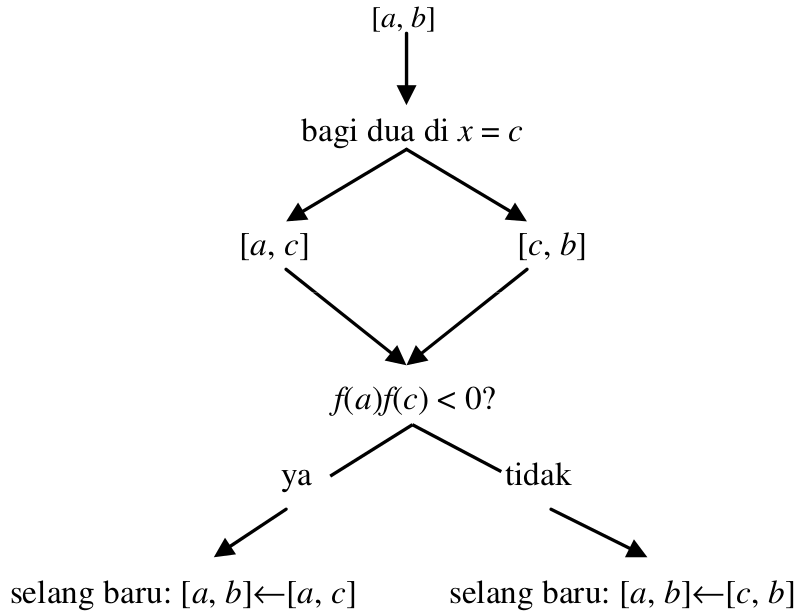
\includegraphics[width=0.7\linewidth]{img/img05.png}
	\end{center}
\end{frame}

\begin{frame}
	\begin{itemize}
		\item Proses pembagian selang $ [a, b] $ dengan metode bagidua
	\end{itemize}
	\begin{center}
		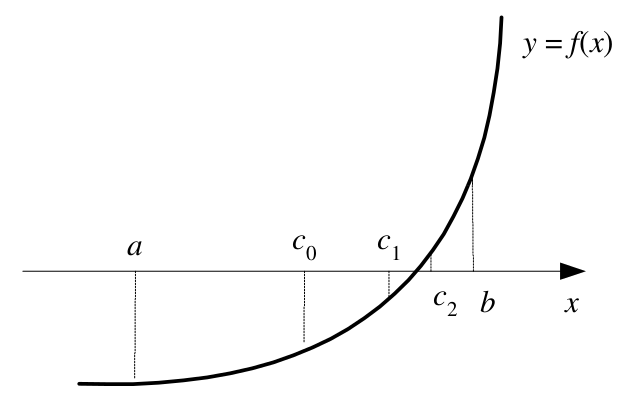
\includegraphics[width=0.7\linewidth]{img/img06.png}
	\end{center}
\end{frame}

\begin{frame}
	Kondisi berhenti iterasi dapat dipilih salah satu dari tiga kriteria berikut:
	\begin{enumerate}
		\item Lebar selang baru: $|a - b| < \varepsilon$ , yang dalam hal ini $\varepsilon$ adalah nilai toleransi lebar selang yang mengurung akar.
		\item Nilai fungsi di hampiran akar: $ f(c) < \mu $ , yang dalam hal ini $\mu$ adalah nilai yang sangat kecil mendekati 0.
		\item Galat relatif hampiran akar: $ |(c_{baru} - c_{lama}) / c_{baru}| < \delta $, yang dalam hal ini $\delta$ adalah galat relatif hampiran yang diinginkan.
	\end{enumerate}
\end{frame}

\begin{frame}
	\frametitle{Contoh 1}
	\begin{itemize}
		\item Temukan akar $ f(x) = e^x - 5x^2 $ di dalam selang $ [0, 1] $ dan $ \varepsilon = 0.00001 $.
		\item Penyelesaian:\\Kita lakukan prosedure metode bagi dua dalam bahasa pemrograman python !
	\end{itemize}
\end{frame}

\begin{frame}
	\frametitle{Kasus yang mungkin terjadi pada penggunaan metode bagidua}
	\begin{enumerate}
		\item Jumlah akar lebih dari satu
		\begin{itemize}
			\item Bila dalam selang [a, b] terdapat lebih dari satu akar (banyaknya akar ganjil), hanya satu buah akar yang dapat ditemukan
			\item Cara mengatasinya: gunakan selang [a,b] yang cukup kecil yang memuat hanya satu buah akar.
		\end{itemize}
		\item Akar ganda
		\begin{itemize}
			\item Metode bagidua tidak berhasil menemukan akar ganda. Hal ini disebabkan karena tidak terdapat perbedaan tanda di ujung-ujung selang yang baru
			\begin{multicols}{2}
				\item Contoh: $ f(x) = (x - 3)^2 = (x-3)(x-3) $, mempunyai dua akar yang sama, yaitu $ x = 3 $
				\columnbreak
				\begin{center}
					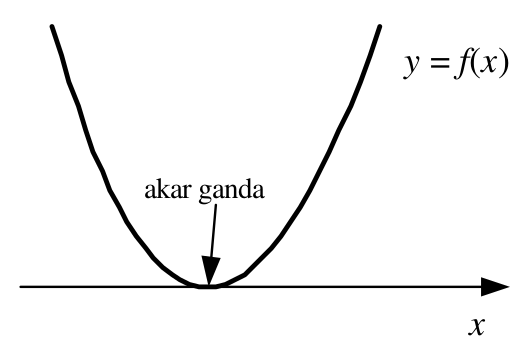
\includegraphics[width=\linewidth]{img/img09}
				\end{center}
			\end{multicols}
		\end{itemize}
	\end{enumerate}
\end{frame}

\begin{frame}
	\frametitle{Kasus yang mungkin terjadi pada penggunaan metode bagidua}
	\begin{enumerate}
		\setcounter{enumi}{2}
		\item Singularitas
		\begin{itemize}
			\item Pada titik singular, nilai fungsinya tidak terdefinisi. Bila selang [a, b] mengandung titik singular, iterasi metode bagidua tidak pernah berhenti. Penyebabnya, metode bagidua menganggap titik singular sebagai akar karena iterasi cenderung konvergen. Yang sebenarnya, titik singular bukanlah akar, melainkan akar semu.
			\begin{multicols}{2}
				\item Cara mengatasinya: periksa nilai $ |f(b) - f(a)| $. Jika $ |f(b) - f(a)| $ konvergen ke nol, akar yang dicari pasti akar sejati, tetapi jika $ |f(b) - f(a)| $ divergen, akar yang dicari merupakan titik singular (akar semu).
				\columnbreak
				\begin{center}
					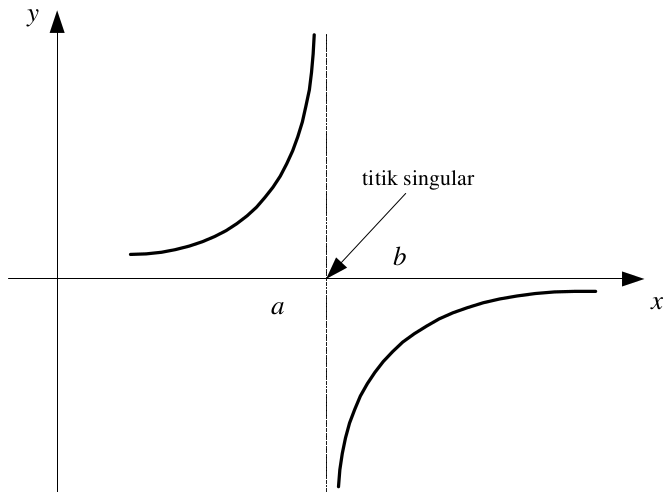
\includegraphics[width=\linewidth]{img/img08}
				\end{center}
			\end{multicols}
		\end{itemize}
	\end{enumerate}
\end{frame}

\subsection{Metode Regula-Falsi}

\begin{frame}
	\frametitle{Metode Regula-Falsi\\(False Position Method)}
	\begin{itemize}
		\item Kelemahan metode bagidua: kecepatan konvergensinya sangat lambat.
		\item Kecepatan konvergensi dapat ditingkatkan bila nilai $ f(a) $ dan $ f(b) $ juga turut diperhitungkan.
		\item Logikanya, bila $ f(a) $ lebih dekat ke nol daripada $ f(b) $ tentu akar lebih dekat ke $ x = a $ daripada ke $ x = b $.
		\item Metode yang memanfaatkan nilai $ f(a) $ dan $ f(b) $ ini adalah \textbf{metode regula-falsi} (bahasa Latin) atau \textbf{metode posisi palsu}. (\textit{false position method})
	\end{itemize}
\end{frame}

\begin{frame}
	\frametitle{Metode Regula-Falsi\\(False Position Method)}
	\begin{center}
		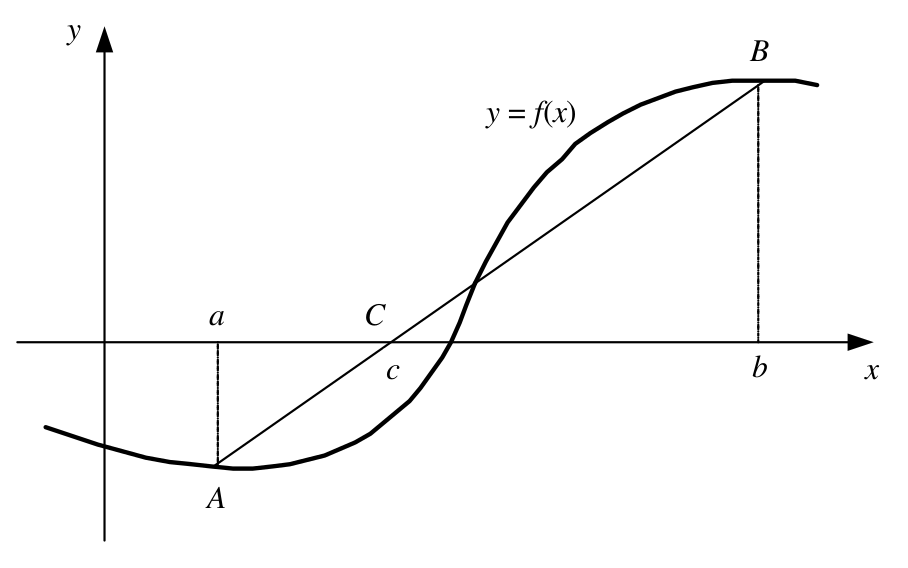
\includegraphics[width=0.6\linewidth]{img/img10}
	\end{center}
	\begin{itemize}
		\item[] gradien garis AB = gradien garis BC
		\[ \frac{f(b) - f(a)}{b - a} = \frac{f(b) - 0}{b - c} \rightarrow c = b - \frac{f(b)(b-a)}{f(b)-f(a)}\]
	\end{itemize}
\end{frame}

\begin{frame}
	\frametitle{Contoh 1}
	\begin{itemize}
		\item Temukan akar $ f(x) = e^x - 5x^2 $ di dalam selang $ [0, 1] $ dan $ \varepsilon = 0.00001 $.
		\item Penyelesaian:\\Kita lakukan prosedure metode regula falsi dalam bahasa pemrograman python !
	\end{itemize}
\end{frame}

\begin{frame}
	\frametitle{Metode Regula-Falsi\\(False Position Method)}
	\begin{itemize}
		\item Secara umum, iterasi metode regula-falsi lebih cepat daripada iterasi metode bagidua
		\item Tetapi, ada kemungkinan iterasi metode regula falsi lebih lambat
		\item Kasus seperti ini akan terjadi bila kurva fungsinya cekung (konkaf) di dalam selang $ [a, b] $.
		\item Akibatnya, garis potongnya selalu terletak di atas kurva atau selalu terletak di bawah kurva.
	\end{itemize}
\end{frame}

\begin{frame}
	\frametitle{Metode Regula-Falsi\\(False Position Method)}
	\begin{center}
		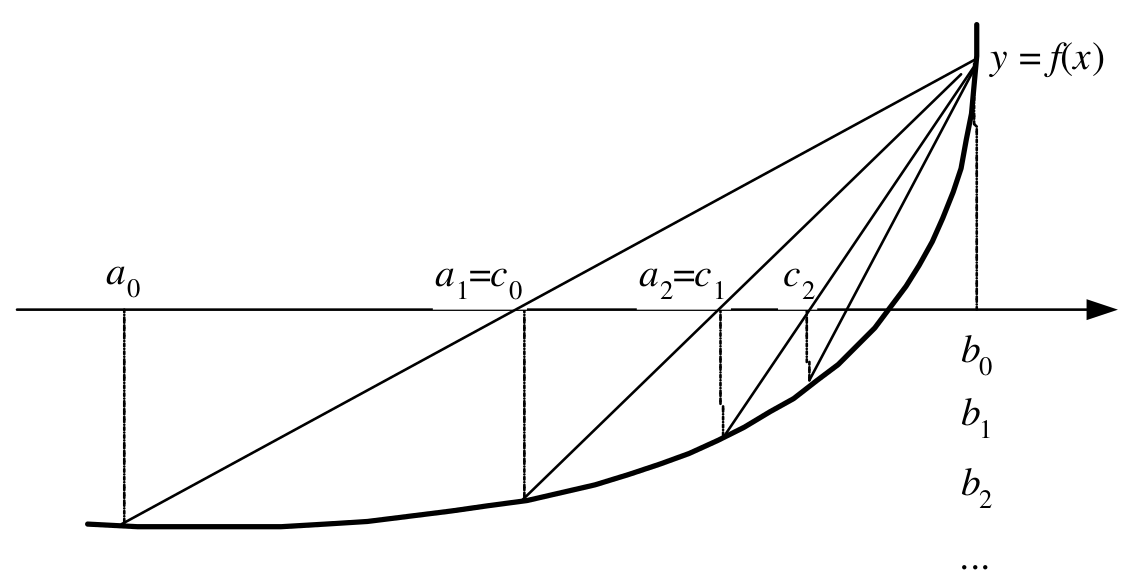
\includegraphics[width=0.6\linewidth]{img/img11}
	\end{center}
\end{frame}

\subsection{Metode Modified \left( \left( Regula-Falsi}

\begin{frame}
	\frametitle{Perbaikan Metode Regula-Falsi \\ (Modified False Position Method)}
	\begin{itemize}
		\item Tentukan titik ujung selang yang tidak berubah (jumlah perulangan $ > $ 1) yang kemudian menjadi titik mandek.
		\item Nilai f pada titik mandek itu diganti menjadi setengah kalinya
		\begin{center}
			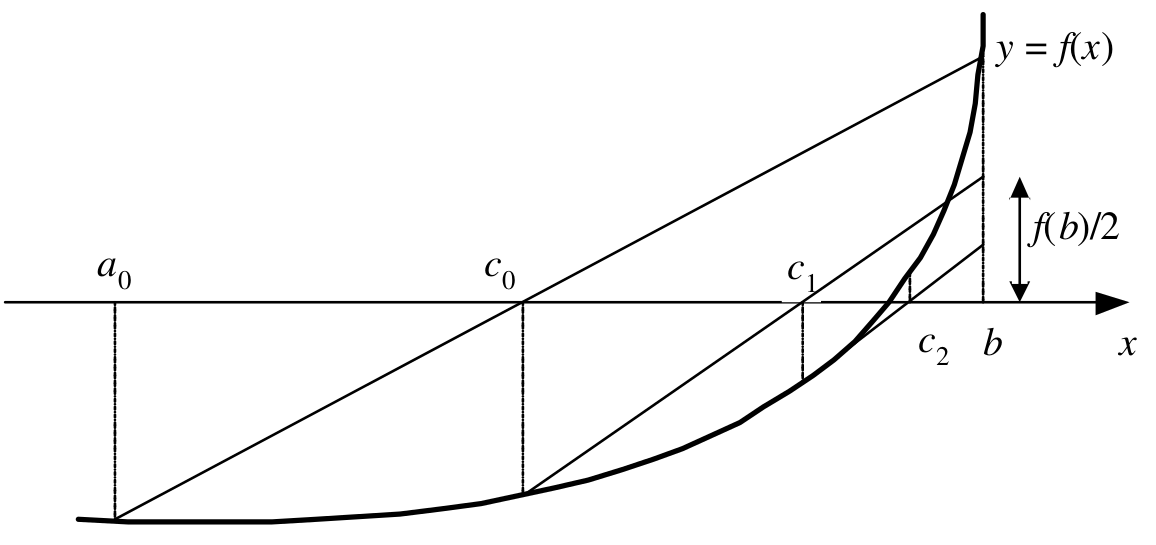
\includegraphics[height=0.5\textheight]{img/img12}
		\end{center}
	\end{itemize}
\end{frame}

\begin{frame}
	\frametitle{Contoh 1}
	\begin{itemize}
		\item Temukan akar $ f(x) = e^x - 5x^2 $ di dalam selang $ [0, 1] $ dan $ \varepsilon = 0.00001 $.
		\item Penyelesaian:\\Kita lakukan prosedure metode modified regula falsi dalam bahasa pemrograman python !
	\end{itemize}
\end{frame}

\section{Metode Terbuka}

\begin{frame}
	\frametitle{Metode Terbuka}
	\begin{itemize}
		\item Tidak memerlukan selang yang mengurung akar.
		\item Hanya memerlukan tebakan awal akar atau dua buah tebakan yang tidak mengurung akar.
		\item Hampiran akar didasarkan pada hampiran akar sebelumnya melalui prosedur iterasi.
		\item Iterasi bisa konvergen, bisa juga divergen.
		\item Jika iterasi konvergen, prosesnya sangat cepat dibandingkan metode tertutup.
	\end{itemize}
\end{frame}

\begin{frame}
	\frametitle{Metode Terbuka}
	Yang termasuk ke dalam metode terbuka:
	\begin{enumerate}
		\item Metode iterasi titik-tetap (fixed-point iteration)
		\item Metode Newton-Raphson
		\item Metode secant
	\end{enumerate}
\end{frame}

\subsection{Metode Iterasi Titik-Tetap (Fix-point Iteration))}

\begin{frame}
	\frametitle{Metode Iterasi Titik-Tetap\\(Fix-point Iteration)}
	\begin{itemize}
		\item Metode ini kadang-kadang dinamakan juga \textbf{metode iterasi sederhana}, \textbf{metode langsung}, atau \textbf{metode sulih beruntun}.
		\item Susunlah persamaan $ f(x) = 0 $ menjadi bentuk $ x = g(x) $. Lalu, bentuklah menjadi prosedur iterasi
		\[ x_{r+1} = g(x_r);~r = 0,1,2,3,\dots \]
		\item Terkalah sebuah nilai awal $ x_0 $ , lalu hitung $ x_1 $ , $ x_2 $ , $ x_3 $ , $ \dots $ yang mudah-mudahan konvergen ke akar sejati.
		\item Kondisi berhenti iterasi dinyatakan bila
		\[ |x_{r+1} - x_r | < \varepsilon \text{ atau } \left| \frac{x_{r+1} - x_r}{x_{r+1}} \right| < \delta\]
	\end{itemize}
\end{frame}

\begin{frame}
	\frametitle{Contoh 2}
	\begin{itemize}
		\item Carilah akar persamaan $ f(x) = x^2 – 2x – 3 = 0 $ dengan metode iterasi titik-tetap. Gunakan $\varepsilon$ = 0.000001.
		\item Ada beberapa kemungkinan prosedur iterasi yang dapat dibentuk
	\end{itemize}
\end{frame}

\begin{frame}
	\frametitle{Prosedur 1}
	\begin{enumerate}
		\item Ubah bentuk persamaannya
		\begin{align*}
		x^2 - 2x - 3 &= 0 \\
		x^2 &= 2x + 3 \\
		x &= \sqrt{2x + 3}
		\end{align*}
		\item Dalam hal ini, $ g(x) = \sqrt{2x + 3} $.
		\item Prosedur iterasinya adalah $ x_{r+1} = \sqrt{2x_r + 3} $. \item Ambil terkaan awal $ x_0 $ = 4
		\item Mari kita lakukan proses komputasinya dengan python.
	\end{enumerate}
\end{frame}

\begin{frame}
	\frametitle{Prosedur 2}
	\begin{enumerate}
		\item Ubah bentuk persamaannya
		\begin{align*}
		x^2 - 2x - 3 &= 0 \\
		x(x-2) &= 3 \\
		x &= 3/(x-2)
		\end{align*}
		\item Dalam hal ini, $ g(x) = 3/(x-2) $.
		\item Prosedur iterasinya adalah $ x_{r+1} = 3/(x_r-2) $.
		\item Ambil terkaan awal $ x_0 $ = 4
		\item Mari kita lakukan proses komputasinya dengan python.
	\end{enumerate}
\end{frame}

\begin{frame}
	\frametitle{Prosedur 3}
	\begin{enumerate}
		\item Ubah bentuk persamaannya
		\begin{align*}
		x^2 - 2x - 3 &= 0 \\
		2x &= x^2 - 3 \\
		x &= (x^2 - 3)/2
		\end{align*}
		\item Dalam hal ini, $ g(x) = (x^2 - 3)/2 $.
		\item Prosedur iterasinya adalah $ x_{r+1} = ({x_r}^2 - 3)/2 $.
		\item Ambil terkaan awal $ x_0 $ = 4
		\item Mari kita lakukan proses komputasinya dengan python.
	\end{enumerate}
\end{frame}

\begin{frame}
	\frametitle{Kriteria Konvergensi}
	\begin{itemize}
		\item Kadang-kadang iterasi konvergen, kadang-kadang ia divergen.
		\item Adakah suatu 'tanda' bagi kita untuk mengetahui kapan suatu iterasi konvergen dan kapan divergen?
		\item Terdapat suatu teorema yang intisarinya mengatakan bahwa syarat konvergen adalah $ |g'(x_0)| < 1 $ yang mana $ x_0 $ adalah titik awal.
	\end{itemize}
\end{frame}

\begin{frame}
	\frametitle{Analisis Contoh 2}
	\begin{enumerate}
		\item Prosedur iterasi pertama $ x_{r+1} = \sqrt{2x_r + 3} $
		\[ g(x) =  \sqrt{2x_r + 3} \rightarrow g'(x) =  \frac{1}{2\sqrt{2x_r + 3}} \]
		\item[] Pengambilan tebakan awal $ x_0 = 4 $ akan menghasilkan iterasi yang konvergen sebab
		\[ |g'(4)| = |1 / [2 \sqrt{(8+3)}]| = 0.1508 < 1\]
	\end{enumerate}
\end{frame}

\begin{frame}
	\frametitle{Analisis Contoh 2}
	\begin{enumerate}
		\item Prosedur iterasi kedua $ x_{r+1} = 3/(x_r - 2) $
		\[ g(x) =  3/(x - 2) \rightarrow g'(x) =  -3/(x - 2)^2 \]
		\item[] Pengambilan tebakan awal $ x_0 = 4 $ akan menghasilkan iterasi yang konvergen sebab
		\[ |g'(4)| = |-3/(4-2)^2| = 0.75 < 1\]
	\end{enumerate}
\end{frame}

\begin{frame}
	\frametitle{Analisis Contoh 2}
	\begin{enumerate}
		\item Prosedur iterasi ketiga $ x_{r+1} = ({x_r}^2 - 3)/2 $
		\[ g(x) = ({x}^2 - 3)/2 \rightarrow g'(x) =  x \]
		\item[] Pengambilan tebakan awal $ x_0 = 4 $ akan menghasilkan iterasi yang konvergen sebab
		\[ |g'(4)| = |4| = 4 > 1\]
	\end{enumerate}
\end{frame}

\begin{frame}
	\frametitle{Kesimpulan}
	Ada 2 hal yang mempengaruhi kekonvergenan prosedur iterasi:
	\begin{enumerate}
		\item Bentuk formula $ x_{r+1} = g(x_r) $
		\item Pemilihan tebakan awal $ x $, yaitu $ x_0 $
	\end{enumerate}
\end{frame}

\begin{frame}
	\frametitle{Contoh 3}
	Gunakan metode lelaran titik-tetap untuk mencari akar persamaan $ x^3 - 3x + 1 $ di dalam selang [1,2]
	\begin{center}
		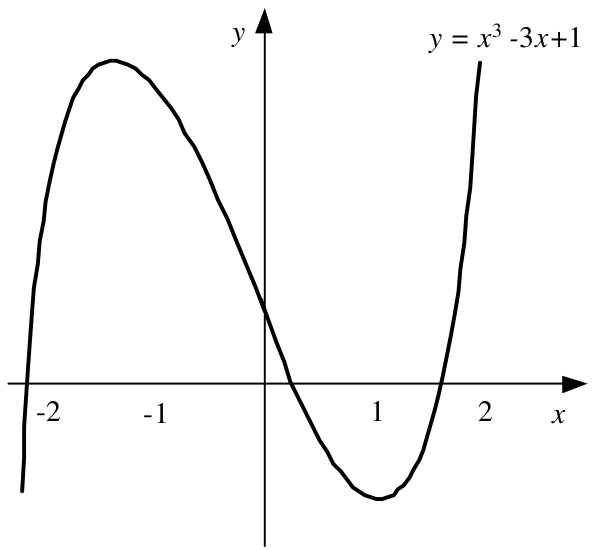
\includegraphics[width=0.5\linewidth]{img/img14}
	\end{center}
\end{frame}

\begin{frame}
	\frametitle{Penyelesaian Contoh 3}
	\begin{enumerate}
		\item $ x_{r+1} = ({x_r}^3 + 1)/3 \rightarrow g'(x) = x^2$ 
		\item $ x_{r+1} = -1/({x_r}^2-3) \rightarrow g'(x) = 2x/(x^2-3)^3$
		\item $ x_{r+1} = 3/x_r - 1/{x_r}^2 \rightarrow g'(x) = (-3x + 2)/x^3 $
		\item[]
		\item[] Kita cek bersama apakah memenuhi kriteria konvergensi atau tidak.
		\item[] Jika ada yang memenuhi kriteria konvergensi, maka kita cari solusinya/akarnya.
	\end{enumerate}
\end{frame}

\subsection{Metode Newton-Raphson}

\begin{frame}
	\frametitle{Metode Newton-Raphson}
	\begin{itemize}
		\item Metode Newton-Raphson yang paling terkenal dan paling banyak dipakai dalam terapan sains dan rekayasa.
		\item Metode ini paling disukai karena konvergensinya paling cepat diantara metode lainnya.
		\item Ada dua pendekatan dalam menurunkan rumus metode Newton-Raphson, yaitu:
		\begin{enumerate}
			\item Penurunan rumus Newton-Raphson secara geometri,
			\item Penurunan rumus Newton-Raphson dengan bantuan deret Taylor
		\end{enumerate}
	\end{itemize}
\end{frame}

\begin{frame}
	\frametitle{Penurunan rumus Newton-Raphson secara geometri}
	\begin{center}
		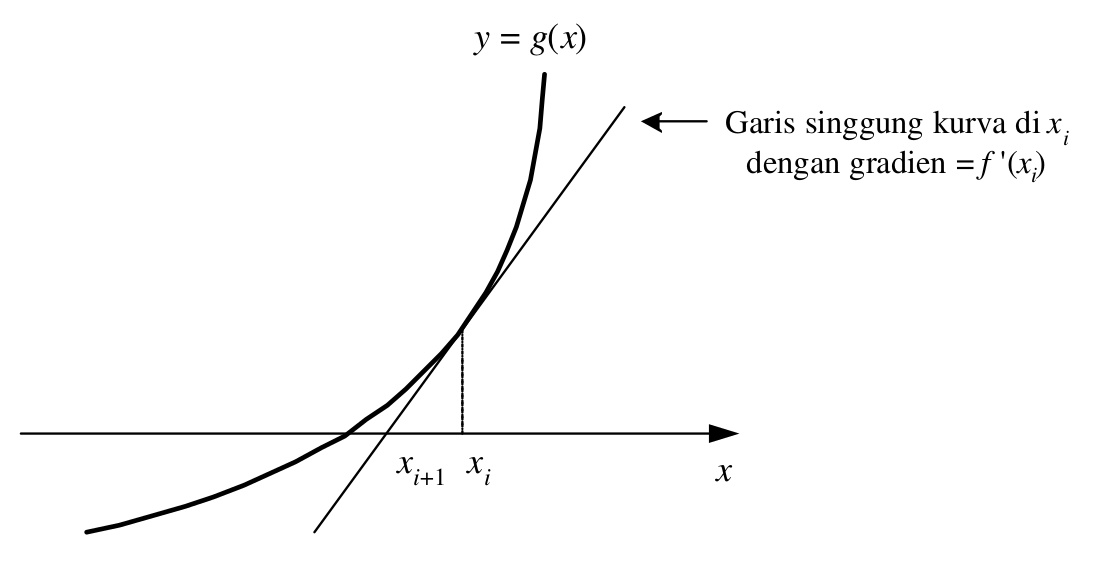
\includegraphics[width=0.6\linewidth]{img/img15}
	\end{center}
	\begin{itemize}
		\item Gradien garis singgung di $ x_r $ adalah
		\begin{align*}
			m = f'(x_r) &= \frac{\Delta y}{\Delta x} = \frac{f(x_r)-0}{x_r - x_{r+1}} \\
			f'(x_r) &= \frac{f(x_r)}{x_r - x_{r+1}} \rightarrow x_{r+1} = x_r - \frac{f(x_r)}{f'(x_r)}, f'(x_r) \neq 0
		\end{align*}
	\end{itemize}
\end{frame}

\begin{frame}
	\frametitle{Penurunan rumus Newton-Raphson dengan bantuan deret Taylor}
	\begin{itemize}
		\item Uraikan $ f(x_{r+1}) $ di sekitar $ x_r $ ke dalam deret Taylor:
		\begin{align*}
			f(x_{r+1}) \approx f(x_r) + (x_{r+1} - x_r)f'(x_r) + \frac{(x_{r+1} - x_r)^2}{2}f''(t),\\
			~x_r<t<x_{r+1}
		\end{align*}
		\item yang bila dipotong sampai suku orde-2 saja menjadi
		\[ f(x_{r+1}) \approx f(x_r) + (x_{r+1} - x_r)f'(x_r) \]
		\item dan karena persoalan mencari akar, maka $ f(x_{r+1} ) = 0 $, sehingga \[ 0 = f(x_r) + (x_{r+1} - x_r)f'(x_r) \text{ atau } x_{r+1} = x_r - \frac{f(x_r)}{f'(x_r)},~f'(x_r) \neq 0\]
	\end{itemize}
\end{frame}

\begin{frame}
	\begin{itemize}
		\item Kondisi berhenti lelaran Newton-Raphson adalah bila
		\[ | x_{r+1} - x_r | < \varepsilon \]
		atau bila menggunakan galat relatif hampiran
		\[ | \frac{x_{r+1} - x_r}{x_{r+1}} | < \delta \]
		dengan $\varepsilon$ dan $\delta$ adalah toleransi galat yang diinginkan
	\end{itemize}
\end{frame}

\begin{frame}
	\frametitle{Contoh 4}
	\begin{itemize}
		\item Hitunglah akar $ f(x) = e^x - 5x^2 $ dengan metode Newton-
		Raphson. Gunakan $\varepsilon = 0.00001$. Tebakan awal akar $ x_0 = 1 $.
		\item[] \textbf{Penyelesaian:}
		\begin{align*}
			f(x) &= e^x - 5x^2\\
			f'(x) &= e^x - 10x
		\end{align*}
		\item[] Prosedur iterasi Newton-Raphson:
		\[ x_{r+1} = x_r - \frac{e^{x_r} - 5{x_r}^2}{e^{x_r} - 10{x_r}} \]
		\item[] Tebakan awal $ x_0 = 1 $
		\item[] Kita lakukan komputasinya dengan python.
	\end{itemize}
\end{frame}

\end{document}